% Minimal TikZ standalone example

\documentclass[tikz,border=10pt]{standalone}

\usepackage{tikz}
\usepackage{tkz-euclide}

\usetikzlibrary{angles,quotes,calc}

\begin{document}
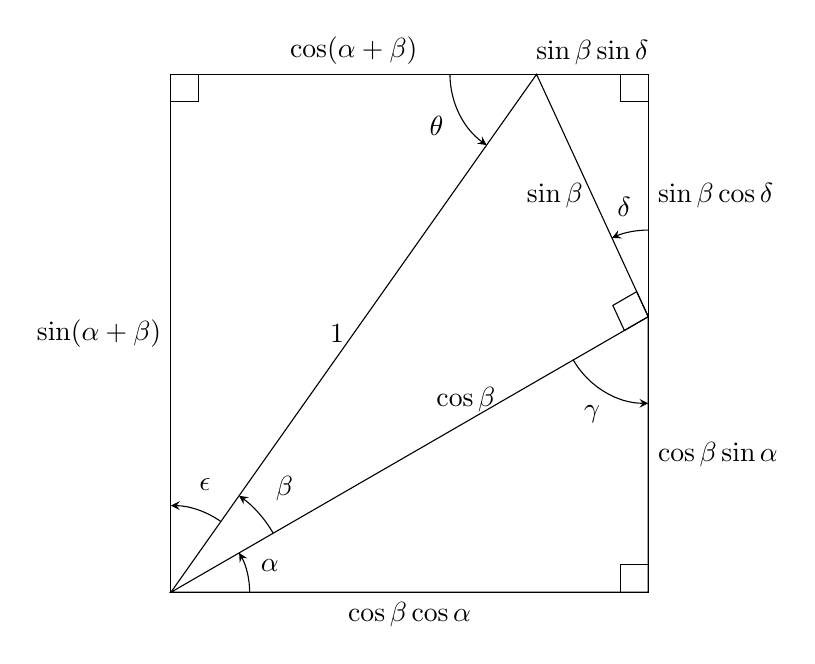
\begin{tikzpicture}[scale=7,>=stealth]

	% angles
	\def\a{30}  % alpha
	\def\b{40}  % beta
	\def\S{1.0}

	% base triangle ABC for alpha (unit hypotenuse)
	\coordinate (A) at (0,0);
	\coordinate (B) at ({\S*cos(\a)},{\S*sin(\a)});
	\coordinate (C) at ({\S*cos(\a)},0);

	% triangle ADB for beta
	\coordinate (D) at ({\S*cos(\a)*cos(\b)},{\S*sin(\a+\b)});

	% engulfing rectangle
	\coordinate (E) at ({\S*cos(\a)},{\S*sin(\a+\b)});
	\coordinate (F) at (0,{\S*sin(\a+\b)});

	% projections
	%\coordinate (G) at ({\S*cos(\a)*cos(\b)},0);

	% triangle sides
	\draw (A) -- (B) -- (C) -- cycle;
	\draw (A) -- (D) -- (B);
	%\draw[dashed] (D) -- (G);

	% rectangle
	\draw (A) rectangle (E);

	% annotations
	\node[left] at ($(A)!0.5!(D)$) {$1$};

	\node[left] at ($(A)!0.7!(B)$) {$\cos\beta$};
	\node[left] at ($(D)!0.5!(B)$) {$\sin\beta$};

	\node[below]  at ($(A)!0.5!(C)$) {$\cos\beta \cos \alpha$};
	\node[right]  at ($(B)!0.5!(C)$) {$\cos\beta \sin \alpha$};

	\node[right]  at ($(E)!0.5!(B)$) {$\sin\beta \cos \delta$};
	\node[above]  at ($(D)!0.5!(E)$) {$\sin\beta \sin \delta$};

	\node[above] at ($(F)!0.5!(D)$) {$\cos(\alpha+\beta)$};
	\node[left] at ($(A)!0.5!(F)$) {$\sin(\alpha+\beta)$};

	% angle alpha
	\pic[draw, ->, "$\alpha$", angle eccentricity=1.3, angle radius=1cm]
	{angle = C--A--B};

	% angle beta
	\pic[draw, ->, "$\beta$", angle eccentricity=1.3, angle radius=1.5cm]
	{angle = B--A--D};

	% angle gamma
	\pic[draw, ->, "$\gamma$", angle eccentricity=1.3, angle radius=1.1cm]
	{angle = A--B--C};

	% angle delta
	\pic[draw, ->, "$\delta$", angle eccentricity=1.3, angle radius=1.1cm]
	{angle = E--B--D};

	% angle epsilon
	\pic[draw, ->, "$\epsilon$", angle eccentricity=1.3, angle radius=1.1cm]
	{angle = D--A--F};

	% angle theta
	\pic[draw, ->, "$\theta$", angle eccentricity=1.3, angle radius=1.1cm]
	{angle = F--D--A};

	% right angles
	\tkzMarkRightAngle[size=0.05](D,B,A)
	\tkzMarkRightAngle[size=0.05](B,C,A)
	\tkzMarkRightAngle[size=0.05](D,E,B)
	\tkzMarkRightAngle[size=0.05](A,F,D)

\end{tikzpicture}
\end{document}
